% !TeX document-id = {a836f75a-a0c6-4045-88b1-6cb4916dad52}
% !TeX TXS-program:compile = txs:///pdflatex/[--shell-escape]
% !TeX TXS-program:bibliography = txs:///biber

\documentclass[]{scrreprt}

\usepackage[backend=biber]{biblatex}
\usepackage[swedish,english]{babel}
\usepackage[utf8]{inputenc}
\usepackage{minted}
\usepackage{graphicx}
\usepackage[iso]{datetime}

%\usepackage[hidelinks]{hyperref}
\usepackage{bookmark}
\usepackage{lastpage}
\usepackage{subcaption}
\usepackage{accsupp}
\usepackage{attachfile}
\usepackage{rotating}
\usepackage{pdflscape}
\usepackage{siunitx}


\usepackage{etoolbox}
\makeatletter
\patchcmd{\scr@startchapter}{\if@openright\cleardoublepage\else\clearpage\fi}{}{}{}
\makeatother
% roman numeral
\newcommand{\RON}[1]{%
	\textup{\uppercase\expandafter{\romannumeral#1}}%
}

% Title Page
\title{Roadster - R1}
\author{Gardström Emil \and Wallin Dennis}
\subtitle{Beräkningsvetenskap \RON{1}}
\titlehead{\Large Uppsala Universitet\hfill KandMa, Grupp \#}

%\addbibresource{\jobname.bib}
\begin{document}
\maketitle
\selectlanguage{english}
%\begin{abstract}
%
%\end{abstract}
\selectlanguage{swedish}
\chapter{Inledning}
\chapter{Resultat}
Vi ser att den bästa den bästa hastigheten att köra vid är \SI{28.7}{\kilo\meter\per\hour},varvid man kan köra \SI{659.48}{\kilo\meter}.
% Fix, this looks really bad
\begin{sidewaysfigure}
	\caption{Utskrift från \textit{s.m}}
	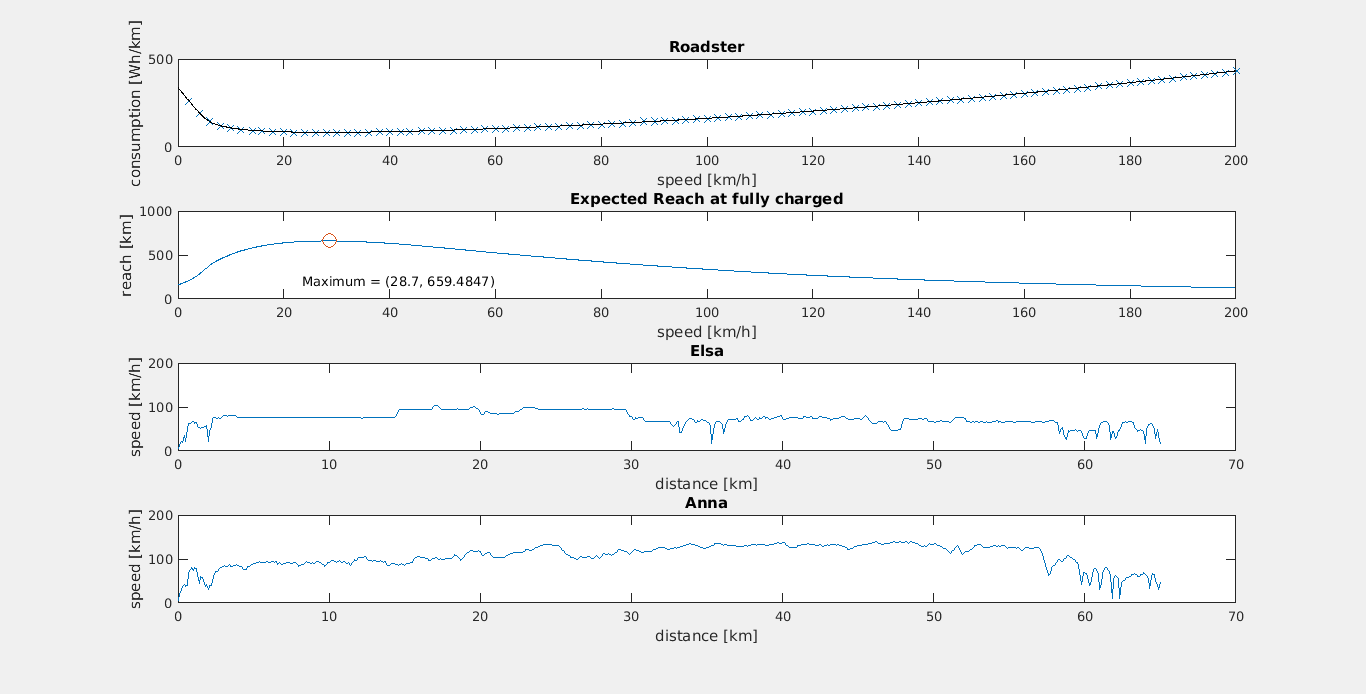
\includegraphics[width=1.2\textwidth]{/home/localsys/projects/uu-bervet1/roadster/part1.png}
\end{sidewaysfigure}
\appendix
\newpage
\fvset{showspaces}
\renewcommand\FancyVerbSpace{\textcolor{white}{\char32}}
% Patch minted/fancyvrb nos
\newcommand\emptyaccsupp[1]{\BeginAccSupp{ActualText={}}#1\EndAccSupp{}}
%default definition is: \def\theFancyVerbLine{\rmfamily\tiny\arabic{FancyVerbLine}}
\let\theHFancyVerbLine\theFancyVerbLine% don't apply our patch to hyperref's version
\def\theFancyVerbLine{\rmfamily\tiny\emptyaccsupp{\arabic{FancyVerbLine}}}
\chapter{s.m}
\attachfile{/home/localsys/projects/uu-bervet1/roadster/s.m}
\inputminted[linenos=true,frame=leftline]{matlab}{/home/localsys/projects/uu-bervet1/roadster/s.m}
%\lstinputlisting[language=matlab,numbers=left,frame=L]{src/simulate.m}
\chapter{velocity.m}
\attachfile{/home/localsys/projects/uu-bervet1/roadster/velocity.m}
\inputminted[linenos=true,,frame=leftline]{matlab}{/home/localsys/projects/uu-bervet1/roadster/velocity.m}
\chapter{consumption.m}
\attachfile{/home/localsys/projects/uu-bervet1/roadster/consumption.m}
\inputminted[linenos=true,,frame=leftline]{matlab}{/home/localsys/projects/uu-bervet1/roadster/consumption.m}
%\chapter{time\_to\_destination.m}
% Fix latex rendering of math
%\attachfile{/home/localsys/projects/uu-bervet1/roadster/time_to_destination.m}
%\inputminted[linenos=true,,frame=leftline,mathescape]{matlab}{/home/localsys/projects/uu-bervet1/roadster/time_to_destination.m}
\end{document}